% Template created by Karol Kozioł (www.karol-koziol.net) for ShareLaTeX

\documentclass[a4paper,9pt]{extarticle}
\usepackage[utf8]{inputenc}
\usepackage[T1]{fontenc}
\usepackage{graphicx}
\usepackage[x11names]{xcolor}
\usepackage{tikz}
\usepackage{fontawesome5}
\usepackage{bm}
\usepackage[most]{tcolorbox}
\usepackage{enumerate}
\usepackage[shortlabels]{enumitem}
\tcbuselibrary{skins,raster,theorems,breakable}

\usepackage{amsmath,amssymb,textcomp}
\usepackage{mathtools}
\everymath{\displaystyle}
\usepackage{multicol}
\usepackage{multirow}
\setlength{\columnseprule}{0pt}
\setlength{\columnsep}{20.0pt}


\usepackage{geometry}
\geometry{a4paper,left=10mm,right=10mm,top=10mm,bottom=15mm}

\newcommand{\trans}[1]{{#1}^{\mathsf{T}}}
\newcommand{\ev}[1]{\mathbb{E}\left[#1\right]}
\newcommand{\unmezz}{\frac{1}{2}}
	\newcommand{\Z}{\mathbb{Z}}
\newcommand{\R}{\mathbb{R}}
\newcommand{\N}{\mathbb{N}}
\newcommand{\T}{\mathbb{T}}
\newcommand{\Tbar}{\overline{\T}}
\newcommand{\Nstar}{\N^{*}}
\newcommand{\Rext}{\overline{\R}}
\newcommand{\io}{\text{ i.o.}}
\newcommand{\equalexpl}[1]{%
	\underset{\substack{\uparrow\\\mathrlap{\text{\vspace{-3cm}\hspace{-1em}#1}}}}{=}}
\newcommand{\dif}{\mathop{}\!\mathrm{d}}
\newcommand{\convas}{\xrightarrow[]{\text{a.s.}}}
\newcommand{\convpr}{\xrightarrow[]{\pr}}
\newcommand{\convd}{\xrightarrow[]{\text{d}}}
\newcommand{\convlp}{\xrightarrow[]{\lp}}
\newcommand{\convw}{\xrightarrow[]{\mathrm{weak}}}
\newcommand{\as}{\text{ a.s.}}
\newcommand{\asstnr}{\sim N(0,1)}
%\def\checkmark{\tikz\fill[scale=0.4](0,.35) -- (.25,0) -- (1,.7) -- (.25,.15) -- cycle;} 
\newcommand{\dx}{\dif x}
\newcommand{\dy}{\dif y}
\newcommand{\dt}{\dif t}
\newcommand{\du}{\dif u}
\newcommand{\ds}{\dif s}
\newcommand{\dw}{\dif\omega}
\newcommand{\dmu}{\dif\mu}
\newcommand{\dpr}{\dif\pr}
\newcommand{\E}{\mathscr{E}}
\newcommand{\B}{\mathscr{B}}
\newcommand{\F}{\mathcal{F}}
\newcommand{\G}{\mathscr{G}}
\newcommand{\HS}{\mathscr{H}}
\newcommand{\Zn}{\mathscr{Z}}
\newcommand{\D}{\mathscr{D}}
\newcommand{\Es}{\mathscr{S}}
\newcommand{\xbar}{\overline{X}}
\newcommand{\rbar}{\overline{\R}}
\newcommand{\ybar}{\overline{Y}}
\newcommand{\xxbar}{\overline{\xbar}}
\newcommand{\xtilde}{\widetilde{X}}
\newcommand{\ifonly}{\underline{if and only if}}
%\newcommand{\Lp}{L^{p}}

\newtcolorbox{riquadro}[1][]{enhanced, breakable,frame style={top color=Aquamarine3,bottom color=Aquamarine3},colback=black!80,coltext=Aquamarine3!50,title=#1,fonttitle=\bfseries,halign title=center,coltitle=black!80}
\makeatletter
\renewcommand*{\maketitle}{%
	\noindent
	\begin{minipage}{0.4\textwidth}
		
\begin{tikzpicture}
			\node[rectangle,rounded corners=6pt,inner sep=10pt,fill=SteelBlue4,text width= 0.95\textwidth] {\color{white}\Huge \@title};
		\end{tikzpicture}
	\end{minipage}
	\hfill
	\begin{minipage}{0.55\textwidth}
		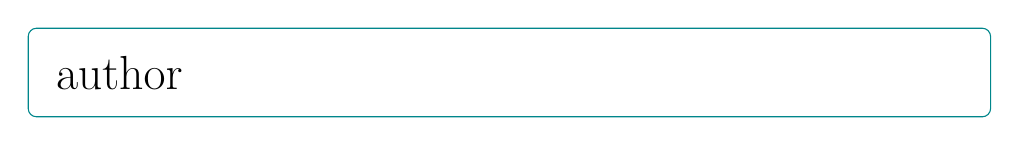
\begin{tikzpicture}
			\node[rectangle,rounded corners=3pt,inner sep=10pt,draw=Turquoise4,text width= 0.95\textwidth] {\LARGE \@author};
		\end{tikzpicture}
	\end{minipage}
}%
\makeatother
\newtcbtheorem[number within=section]{myproof}{Proof}{
	enhanced, sharp corners, breakable,
	colframe=LightSalmon1, coltitle=black, colbacktitle=gray!24,
	coltext=LightSalmon1!60,
	colback=black!80,
	rounded corners,
	fonttitle=\bfseries,
	separator sign={:},
	theorem hanging indent/.try=0pt,
}{ciao}

% custom section
\usepackage[explicit]{titlesec}
\newcommand*\sectionlabel{}
\newcommand{\pr}{\mathbb{P}}
\newcommand{\mbf}[1]{\mathbf{#1}}

\titleformat{\section}
{\gdef\sectionlabel{}
	\normalfont\rmfamily\Large\bfseries}
{\gdef\sectionlabel{\thesection\ }}{0pt}
{
	\noindent
	\begin{tikzpicture}
		\node[rectangle,rounded corners=3pt,inner sep=4pt,fill=Turquoise4,text width= 0.95\columnwidth] {\color{white}\sectionlabel#1};
	\end{tikzpicture}
}
\titlespacing*{\section}{0pt}{0pt}{-10pt}
\newcommand*\subsectionlabel{}
\titleformat{\subsection}
{\gdef\subsectionlabel{}
	\normalfont\rmfamily\Large\bfseries}
{\gdef\subsectionlabel{\thesubsection\ }}{0pt}
{
	\noindent
	\begin{tikzpicture}
		\node[rectangle,inner sep=4pt,fill=Turquoise4!60!black,rounded corners=3pt,text width= 0.9\columnwidth] {\color{white}\subsectionlabel#1};
	\end{tikzpicture}
}
\titlespacing*{\subsection}{0pt}{0pt}{0pt}

% custom footer
\usepackage{fancyhdr}
\makeatletter
\pagestyle{fancy}
\fancyhead{}
\fancyfoot[C]{\footnotesize \textcopyright\ \@date\ \ \@author}
\renewcommand{\headrulewidth}{0pt}
\renewcommand{\footrulewidth}{0pt}
\makeatother



\title{Il Diocane: Introduction to Data Mining Cheatsheet}
\author{\faSynagogue\;Kotatsu, the Bringer of Jewishness\;\faMenorah}
\date{\today}



\begin{document}
	
\maketitle
	
\begin{multicols*}{2}
\section{Similarity and dissimilarity}
\begin{riquadro}
	Entropy:
	\begin{equation*}
		H(X)=-\sum_{i=1}^{n}p_{i}\log_{2}p_i.
	\end{equation*}
	Sample entropy:
	\begin{equation*}
		H(X)=-\sum_{i=1}^{n}\frac{m_{i}}{m}\log_{2}\frac{m_{i}}{m}
	\end{equation*}
	Mutual information:
	\begin{equation*}
		I(X,Y)=H(X)+H(X)-H(X,Y)
	\end{equation*}
	where $H(X,Y)=-\sum_{i=1}^{n}\sum_{j=1}^{n}p_{ij}\log_{2}p_{ij}$. For discrete variables the maximum mutual information is 
	\begin{equation*}
		\log_{2}(\min\{n_{x},n_{y}\})
	\end{equation*}
	where $n_{x}$ is th number of values that $X$ can take.
\end{riquadro}
We can combine similarities with
\begin{equation*}
	\mathrm{similarity}(\mathbf{x},\mathbf{y})=\frac{\sum_{k=1}^{n}w_k\delta_{k}s_{k}((\mathbf{x},\mathbf{y}))}{\sum_{k=1}^{n}w_k\delta_{k}}
\end{equation*}
with
\begin{equation*}
	\delta_{k}=\begin{cases}
		0&\text{\footnotesize\parbox{2.5cm}{if both attribute are asymmetric AND they are both zero or if one of them is missing}}\\
		1&\text{\footnotesize otherwise}
	\end{cases}
\end{equation*}
\section{Clustering}
\begin{riquadro}
	Number of possible clusters:
	\begin{equation*}
		B(n)=\sum_{k=0}^{\infty}\frac{k^{n}}{k!}
	\end{equation*}
	Sum of squared error (what we want to minimize):
	\begin{equation*}
		\mathrm{SSE}=\sum_{i-1}^{K}\sum_{x\in C_i}\mathsf{dist}(m_i,x)^{2}.
	\end{equation*}
\end{riquadro}
So we are trying to minimize the loss function, for the centroids of $K$ clusters $\mathbf{c}=(c_1,\ldots,c_K)$:
\begin{equation*}
	\mathrm{L}(\mathbf{c})=\sum_{i=1}^{n}\min_{j=1,\ldots,K}\lVert x_{i}-c_{j}\rVert^{2}_{2}.
\end{equation*}
We alternate between
\begin{itemize}
	\item updating $z_{i}=\arg\min_{j=1,\ldots,k}\lVert x_{i}-c_{j}\rVert^{2}_{2}$ (maps point $x_{i}$ to a cluster j);
	\item updating $c_{j}=\frac{1}{\left|\{i|z_{i}=j\}\right|}\sum_{i|z_{i}=j}x_{i}$ (recomputes the cluster centroids)
\end{itemize}
\begin{riquadro}[Unsupervised measures of cluster validity]
	\begin{itemize}
	\item 	\textbf{Cohesion}: within-cluster sum of squares (SSW)
	\begin{equation*}
		\mathrm{SSW}=\sum_{i=1}^{K}\sum_{x\in C_i}(x-m_{i})^{2}.
	\end{equation*}
	\item \textbf{Separation}: between-cluster sum of squares (SSB)\\
	\begin{equation*}
		\mathrm{SSB}=\sum_{i}|C_{i}|(m-m_i)^{2}
	\end{equation*}
	where $|C_{i}|$ is the size of cluster $i$ and $m$ is the global centroid.\\
	\item \textbf{Silhouette coefficient}: for a point $P_{i}$ calculate the avg distance $a$ to the points of the cluster and the minimum avg distance $b$ to the points of another cluster. The silhouette coefficient is
	\begin{equation*}
		s=\frac{b-a}{\max\{a,b\}}.
	\end{equation*}
	\end{itemize}
\end{riquadro}
\begin{riquadro}[Supervised measures of cluster validity]
	\begin{itemize}
	\item 	\textbf{Label probability per cluster}:
	\begin{equation*}
		p_{ij}=\frac{m_{ij}}{m_{j}}
	\end{equation*}
	where $m_{j}$: size of cluster $j$ and $m_{ij}$: number of elements of cluster $j$ that are labelled $i$.
	\item \textbf{Entropy of cluster $j$}:
	\begin{equation*}
		h_{j}=\sum_{i=1}^{L}p_{ij}\log_{2}p_{ij}.
	\end{equation*}
\textbf{Total entropy}:
	\begin{equation*}
		h=\sum_{j=1}^{K}\frac{m_{j}}{m}h_{j}.
	\end{equation*}
	\item \textbf{Purity}:
	\begin{equation*}
		\mathrm{purity}_{j}=\max\{p_{ij}\}.
	\end{equation*}
	\textbf{Total purity}:
	\begin{equation*}
		\mathrm{purity}=\sum_{j=1}^{K}\frac{m_{j}}{m}\mathrm{purity}_{j}.
	\end{equation*}
	\item \textbf{Precision}:
	\begin{equation*}
		\frac{TP}{TP+FP}=\frac{m_{ij}}{m_{j}}=p_{ij}.
	\end{equation*}
	\item \textbf{Recall}:
	\begin{equation*}
		\frac{TP}{TP+FN}=\frac{m_{ij}}{m_{i}}.
	\end{equation*}
	\item \textbf{F-measure}:
	\begin{equation*}
		2\cdot\frac{\text{precision}\cdot\text{recall}}{\text{precision}+\text{recall}}.
	\end{equation*}
	\end{itemize}
\end{riquadro}
	Remember that we have
\begin{center}
	\begin{tabular}{|c|c|cc|}
		\cline{3-4}
		\multicolumn{2}{c}{}&\multicolumn{2}{|c|}{cluster}\\
		\cline{3-4}
		\multicolumn{2}{c|}{}&same&different\\
		\hline
		\multirow{2}{*}{\rotatebox[origin=c]{90}{class\hspace*{0.5cm}}}&\rotatebox[origin=c]{90}{same}&$f_{11}$&$f_{10}$\\
		\cline{2-4}
		&\rotatebox[origin=c]{90}{different}&$f_{01}$&$f_{00}$\\
		\hline
	\end{tabular}
\end{center}
\begin{riquadro}[More supervised measures]
	\begin{itemize}
		\item \textbf{Rand statistic}:
		\begin{equation*}
			R=\frac{f_{00}+f_{11}}{f_{00}+f_{01}+f_{10}+f_{11}}.
		\end{equation*}
		\item \textbf{Jaccard coefficient}:
		\begin{equation*}
			J=\frac{f_{11}}{f_{01}+f_{10}+f_{11}}.
		\end{equation*}
		\item \textbf{Adjusted Rand Index}:
		\begin{equation*}
			\mathrm{ARI}=\frac{R(L,C)-\ev{R(L,C)}}{\max\left\{R(L,C),\ev{R(L,C)\right\}}}
		\end{equation*}
		with
		\begin{align*}
			\ev{R(L,C)}&=\frac{\pi(L)\pi(C)}{\frac{n(n-1)}{2}}\\
			\max\left\{R(L,C)\right\}&=\unmezz(\pi(L)-\pi(C))
		\end{align*}
		with $\pi(C)$: number of objects pairs that belong to the same group $C$.
	\end{itemize}
\end{riquadro}
\section{Fuzzy clustering}
We generalize $k$-mean objective function
\begin{equation*}
	\mathrm{SSE}=\sum_{j=1}^{k}\sum_{i=1}^{n}w_{ij}^{p}\mathrm{dist}\left(\mathbf{x}_{i},\mathbf{c}_{j}\right)^{2}.
\end{equation*}
So the procedure is
\begin{enumerate}
	\item choose random weights $w_{ij}$;
	\item until centroids do not change:
	\begin{enumerate}
		\item $\mathbf{c}_{j}=\frac{\sum_{i=1}^{n}w_{ij}\mathbf{x}_{i}}{\sum_{i=1}^{n}w_{ij}}$ (updates centroids);
		\item $w_{ij}=\frac{\left(\frac{1}{\mathrm{dist}(\mathbf{x_{i},\mathbf{c}_{j}})^{2}}\right)^{\frac{1}{p-1}}}{\sum_{q=1}^{k}\left(\frac{1}{\mathrm{dist}(\mathbf{x_{i},\mathbf{c}_{q}})^{2}}\right)^{\frac{1}{p-1}}}$ (updates weights).
	\end{enumerate}
\end{enumerate}
\end{multicols*}
\end{document}